%----------------------------------------------------------------------------------------
%	PACKAGES AND THEMES
%----------------------------------------------------------------------------------------
\documentclass[aspectratio=169,xcolor=dvipsnames]{beamer}
\usetheme{SimplePlusAIC}
\usefonttheme{professionalfonts}

\usepackage{hyperref}
\usepackage{graphicx} % Allows including images
\usepackage{booktabs} % Allows the use of \toprule, \midrule and  \bottomrule in tables
\usepackage{svg} %allows using svg figures
\usepackage{tikz}
\usepackage{makecell}
\newcommand*{\defeq}{\stackrel{\text{def}}{=}}

\newcommand{\ie}{\textit{\fontspec{Times New Roman}i.e.}}
\newcommand{\eg}{\textit{\fontspec{Times New Roman}e.g.}}
\usepackage{natbib}
\usepackage{ulem}
\usepackage{wrapfig}
\usepackage{ragged2e}
\usepackage{bm}
\usepackage[ruled,vlined,linesnumbered]{algorithm2e}
\usepackage{hyperref}
\usepackage{mathtools}
\usepackage{multirow}
\usepackage{pifont}
% \usepackage{enumitem}

%Select the Epilogue font (requires luaLatex or XeLaTex compilers)
\usepackage{fontspec}
\setsansfont{Epilogue}[
    Path=./epilogueFont/,
    Scale=0.9,
    Extension = .ttf,
    UprightFont=*-Regular,
    BoldFont=*-Bold,
    ItalicFont=*-Italic,
    BoldItalicFont=*-BoldItalic
    ]

%----------------------------------------------------------------------------------------
%	TITLE PAGE
%----------------------------------------------------------------------------------------

\title[short title]{Nonparametric Teaching of Implicit Neural Representations} % The short title appears at the bottom of every slide, the full title is only on the title page

\author{Chen Zhang$^{1 *}$, Steven Tin Sui Luo$^{2 *}$, Jason Chun Lok Li$^1$, Yik-Chung Wu$^1$, Ngai Wong$^1$}
\institute{$^1$The University of Hong Kong\newline$^2$The University of Toronto}
% Your institution as it will appear on the bottom of every slide, maybe shorthand to save space


\date{\today} % Date, can be changed to a custom date
%----------------------------------------------------------------------------------------
%	PRESENTATION SLIDES
%----------------------------------------------------------------------------------------

\begin{document}

\begin{frame}[plain]
    % Print the title page as the first slide
    \titlepage
\end{frame}

\begin{frame}{Overview}
    % Throughout your presentation, if you choose to use \section{} and \subsection{} commands, these will automatically be printed on this slide as an overview of your presentation
    \tableofcontents
\end{frame}


%------------------------------------------------
\section{Nonparametric Iterative Machine Teaching}
\begin{frame}
    \LARGE{\centerline{\textbf{Nonparametric Iterative Machine Teaching}}}
\end{frame}
%------------------------------------------------
\subsection{What is Machine Teaching?}
\begin{frame}{What is Machine Teaching?}
\vspace{-2mm}

\justify
Machine teaching (MT)~\cite{zhu2015machine, zhu2018overview} is the study of how to design the \alert{optimal teaching set}, typically with \alert{minimal} examples, so that learners can \textcolor{red}{quickly} learn \alert{target models} based on these examples.
\vspace{1mm}

\justify
It can be considered as an \alert{inverse problem} of machine learning, where \uline{machine learning aims to learn model parameters from a dataset}, while \uline{MT aims to find a minimal dataset from the target model parameters}.

% \vspace{-3mm}

\begin{figure}
  \centering
  \includegraphics[width=0.75\textwidth]{Source/MLvsMT.pdf}
\end{figure}

\end{frame}
%------------------------------------------------
\subsection{What does ``Iterative" mean?}
\begin{frame}{What does ``Iterative" mean?}
\vspace{-2mm}

\justify
Considering the \alert{interaction manner} between teachers and learners, MT can be conducted in either\begin{itemize}
    \item {\color{blue} batch} fashion \cite{zhu2015machine, mansouri2019preference, kumar2021teaching, qian2022teaching} where the teacher is allowed to interact with the learner {\color{red} once}, or 
    \item {\color{blue} iterative} fashion \cite{liu2017iterative, liu2018towards, Liu2021LAST} where an iterative teacher would feed examples {\color{red} sequentially} based on current status of the iterative learner.
\end{itemize}

\begin{figure}
  \centering
  \includegraphics[width=0.75\textwidth]{Source/BatchVSiterative.pdf}
\end{figure}
\end{frame}
%------------------------------------------------
\subsection{What is the difference between ``Parametric" and ``Nonparametric"?}
\begin{frame}{``Parametric" VS. ``Nonparametric"}
\vspace{-4mm}
\justify
{\bf Parametric Teaching} \cite{liu2017iterative, liu2018towards, xu2021locality, wang2021gradient} assumes that $f$ can be represented by a set of parameters $\bm{w}$, \eg, $f(\bm{x})=\langle \bm{w}, \bm{x}\rangle$ with input $\bm{x}$\footnote{\scriptsize The loss $\mathcal{L}$ can be general for different tasks, \eg, square loss for regression and hinge loss for classification.}.
\vspace{-2mm}
\begin{figure}
  \centering
  \includegraphics[width=0.4\textwidth]{comp.pdf}
\end{figure}
\vspace{-2mm}

Parametric assumption results in difficulty when the target models are defined to be \alert{functions without dependency on parameters} (viz. non-closed-form functions). Such a limitation is addressed by {\bf Nonparametric Teaching} \cite{zhang2023nonparametric,zhang2023mint}, which generalizes model space from a finite dimensional one to {\color{red} an infinite dimensional one}.
\end{frame}

%------------------------------------------------
\section{Implicit Neural Teaching (INT)}
\begin{frame}
    \LARGE{\centerline{\textbf{Implicit Neural Teaching (INT)}}}
\end{frame}
%------------------------------------------------
\subsection{Implicit Neural Representations}
\begin{frame}{Implicit Neural Representations}
\justify
\vspace{-2mm}
Implicit neural representation (INR)~\cite{sitzmann2020implicit,tancik2020fourier} focuses on modeling a given signal, which is often discrete, through the use of \alert{an \textcolor{red}{overparameterized} multilayer perceptron (MLP)} such that the signal is accurately fitted by this MLP preserving great details.

\vspace{3mm}

Such an overparameterized MLP inputs \alert{low-dimensional coordinates} of the given signal and outputs corresponding values for each input location, \eg, the MLP maps 2D input coordinates to their respective 8-bit levels for a grayscale image.

\begin{figure}
  \centering
  \includegraphics[width=0.7\textwidth]{Source/INRdemo.pdf}
\end{figure}
\end{frame}

%------------------------------------------------
\subsection{Motivation}
\begin{frame}{Motivation}
    \justify
    The motivation comes from two folds:
    \begin{itemize}
    \item {Lower the training cost and enhance
the \alert{training efficiency} of INR, which is urgently needed when dealing with \alert{high-definition signals}. For instance, consider the case of a 2D grayscale image with a resolution of $1024\times1024$, which leads to a training set comprising $10^6$ pixels}
    \item {Expand the \alert{applicability} of \alert{nonparametric teaching} towards deep learning. ``Nonparametric" is a quite \alert{abstract} concept, which may be of interest for theoretical analysis but \alert{less practical}.}
\end{itemize}
\end{frame}

\begin{frame}{Cont.}
    \justify
    \begin{itemize}
        \item[$\bm{\dagger}$] If we can \alert{connect} nonparametric teaching \alert{to} MLP training, both problems including training efficiency and applicability are addressed. 
        \item[$\bm{\dagger}$] Unfortunately, the evolution of an MLP is typically achieved by \alert{gradient descent on its parameters}, whereas nonparametric teaching involves \alert{functional gradient descent} as the means of function evolution. 
        \end{itemize}

\begin{figure}
    \centering
    \includegraphics[width=0.7\linewidth]{Source/Qbridge.pdf}
\end{figure}
\vspace{-1em}

Bridging this (theoretical + practical) \alert{gap} is of great value and calls for more examination prior to the application of \alert{nonparametric teaching algorithms} in the context of \alert{INR}. \textbf{\textit{Can we do that}}?
\end{frame}

\begin{frame}{Cont.}
\includegraphics[width=\linewidth]{Source/Cbridge.pdf}
\end{frame}

\subsection{Neural Tangent Kernel}
\begin{frame}{Neural Tangent Kernel}
\justify
Neural Tangent Kernel \cite{jacot2018neural,lee2019wide,bietti2019inductive,dou2021training} is a \alert{symmetric and positive definite kernel function}, which is derived from the analysis of the \alert{evolution of a neural network} (the MLP is considered).

\vspace{-1em}
\scriptsize{
\begin{equation}
    K_{\theta^t}(\bm{x}_i,\cdot)=\left\langle\left.\frac{\partial f_{\theta}}{\partial \theta}\right|_{\cdot,\theta^t},\left.\frac{\partial f_{\theta}}{\partial \theta}\right|_{\bm{x}_i,\theta^t} \right\rangle
\end{equation}
}


\centering
\includegraphics[width=0.7\linewidth]{Source/ntk_computation.pdf}
\end{frame}

\subsection{Intuitive Illustration of INT Workflow}
\begin{frame}{Intuitive Illustration of INT Workflow}
\begin{columns}
    \column{0.6\textwidth}
    \centering
    % \vspace{-0.2in}
    \includegraphics[height=7cm]{Source/figure1.pdf}
    \column{0.4\textwidth}
    \justify
    By comparing the \alert{disparity} between the given signal and the current MLP output (a), the nonparametric teacher (b) \alert{selectively chooses} examples (pixels) of the \alert{greatest} disparity (red boxes), instead of a raster scan, to feed to the MLP learner (c) who undergoes learning (\ie, training) (d) and outputs the final (e).
\end{columns}
\end{frame}


%------------------------------------------------
\section{Experiments and Results}
\begin{frame}{Experiments and Results}

\justify
We conduct extensive experiments to validate the \alert{effectiveness} of INT.

\vspace{1mm}
\begin{itemize}
    \item {\bf Toy 2D Cameraman fitting.}
\end{itemize}

\begin{figure}
  \centering
  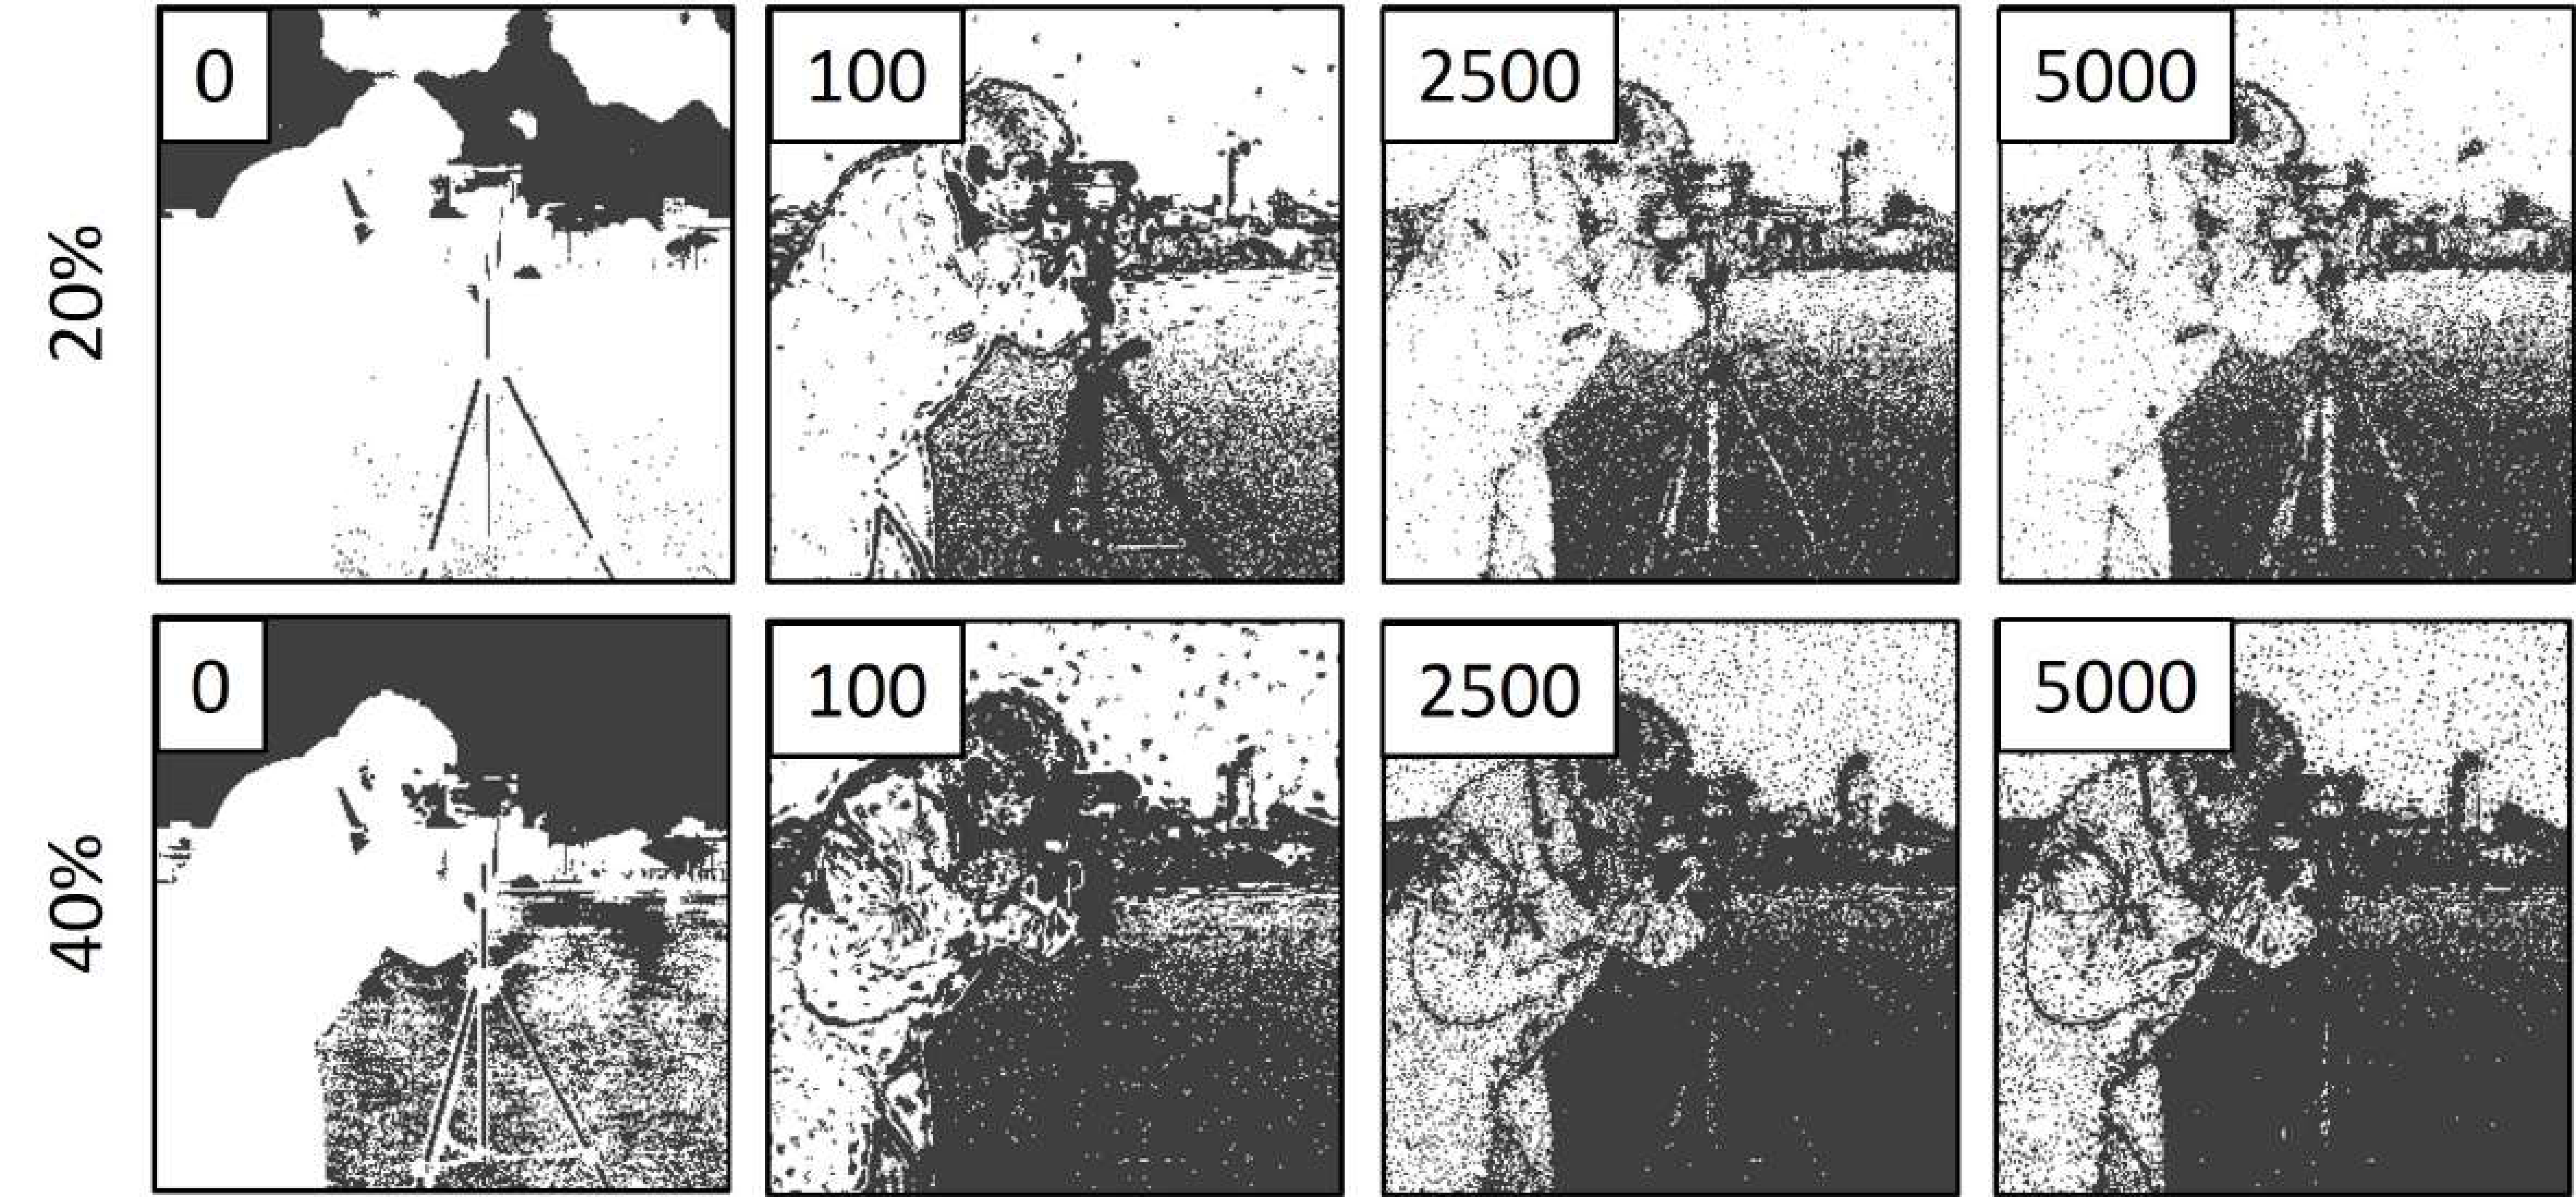
\includegraphics[width=0.6\textwidth]{out/sampling_dynamics_camera.pdf}
  \caption{Progression of INT selected pixels (marked as black) at corresponding iterations when training with INT 20\% (top) and 40\% (bottom).}
\end{figure}
\end{frame}

\begin{frame}{Cont.}
\begin{figure}
\centering
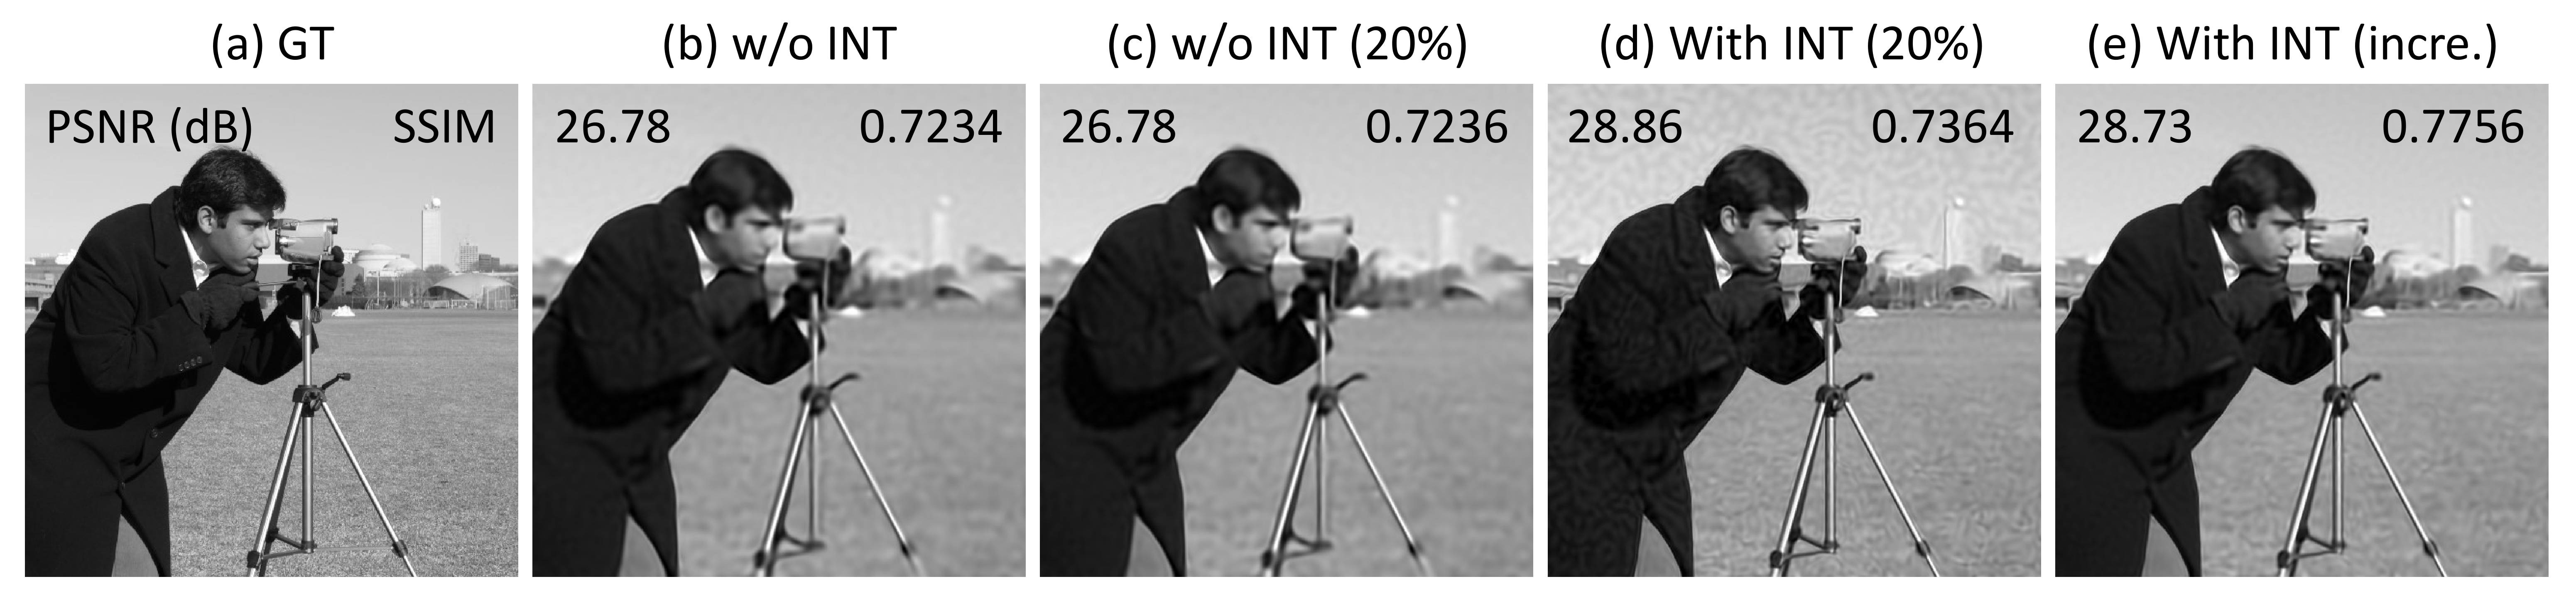
\includegraphics[width=\textwidth]{out/best_pred_summary.pdf}
\caption{Reconstruction quality of SIREN. (b) trains SIREN without (w/o) INT using all pixels. (c) trains it w/o INT using 20\% randomly selected pixels. (d) trains it using INT of 20\% selection rate. (e) trains it using progressive INT (\ie, increasing selection rate progressively from 20\% to 100\%).}
\end{figure}
\end{frame}

\begin{frame}{Cont.}
\vspace{-1mm}
\begin{itemize}
    \item {\bf INT on multiple real-world modalities.}
\end{itemize}


\begin{table}[t]
\centering
\resizebox{.5\linewidth}{!}{
\begin{tabular}{c|c|cc}
\toprule
    INT                           & Modality & Time (s) & PSNR(dB) / IoU(\%) $\uparrow$ \\
    \midrule
    \multirow{4}{*}{\ding{55}}    & Audio  &  23.05 & 48.38$\pm$3.50 \\
                                  &Image   &  345.22   & 36.09$\pm$2.51 \\
                                  &Megapixel   &  16.78K   & 31.82 \\
                                  &3D Shape&  144.58 & 97.07$\pm$0.84 \\
    \midrule
    \multirow{4}{*}{\checkmark}   &Audio    & 15.76 (-31.63\%) & 48.15$\pm$3.39  \\
                                  &Image   &  211.04 (-38.88\%)  & 36.97$\pm$3.59 \\
                                  &Megapixel   &  11.87K (-29.26\%)   & 33.01 \\
                                  &3D Shape& 93.19 (-35.54\%)& 96.68$\pm$0.83\\
    \bottomrule
    \end{tabular}%
    }
\caption{Signal fitting results for different data modalities. The encoding time is measured excluding data I/O latency.}
\label{tab:signal_fitting}
\end{table}

\end{frame}

%------------------------------------------------
\section{Contribution Summary}
\begin{frame}
    \LARGE{\centerline{\textbf{Contribution Summary}}}
\end{frame}
%------------------------------------------------
\begin{frame}{Contributions Summary}

{\bf \color{blue} Main Contribution}: 
\begin{itemize}
\setlength\itemsep{0.1em}
\item We propose \alert{Implicit Neural Teaching} (INT) that novelly interprets \alert{implicit neural representation} (INR) via the theoretical lens of \alert{nonparametric teaching}, which in turn enables the utilization of greedy algorithms from the latter to effectively \alert{bolster the training efficiency} of INRs.
\item We unveil a strong \alert{link} between the evolution of a \alert{multilayer perceptron} (MLP) using gradient descent on its parameters and that of a function using functional gradient descent in \alert{nonparametric teaching}. This connects nonparametric teaching to MLP training, thus expanding the \alert{applicability} of nonparametric teaching towards deep learning. %We further show that the dynamic NTK, derived from gradient descent on the parameters, converges to the canonical kernel of functional gradient descent.
\item We showcase the \alert{effectiveness} of INT through extensive experiments in INR training across multiple modalities. Specifically, INT saves training time  for 1D audio (-31.63\%), 2D images (-38.88\%) and 3D shapes (-35.54\%), while upkeeping its reconstruction quality.
\end{itemize}
\end{frame}

\begin{frame}
    \Huge{\centerline{\textbf{Thank you for listening!}}}
\end{frame}

%------------------------------------------------
\begin{frame}[allowframebreaks]
    \frametitle{References}
    \bibliographystyle{plain}
    {\footnotesize \bibliography{ref.bib}}
\end{frame}

\iffalse

%------------------------------------------------
\subsection{Evolution of an overparameterized MLP}
\begin{frame}{Evolution of an overparameterized MLP}
Given a training set of size $N$ $\{(\bm{x}_i,y_i)|\bm{x}_i\in\mathcal{X},y_i\in\mathcal{Y}\}_N$, the parameter evolves as:
\begin{eqnarray}
	\theta^{t+1}\gets\theta^t-\frac{\eta}{N}\sum_{i=1}^N\nabla_{\theta}\mathcal{L}(f_{\theta^t}(\bm{x}_i),y_i).
\end{eqnarray}
When governed by an extremely small learning rate $\eta$, the update is minute enough over multiple iterations, allowing it to be approximated as a derivative on the time dimension and subsequently transformed into a differential equation:
\begin{eqnarray}
	\frac{\partial\theta^t}{\partial t}=-\frac{\eta}{N}\left[\left.\frac{\partial\mathcal{L}}{\partial f_{\theta}}\right|_{f_{\theta^t},\bm{x}_i}\right]^T_N\cdot \left[\left.\frac{\partial f_{\theta}}{\partial \theta}\right|_{\bm{x}_i,\theta^t}\right]_N.
\end{eqnarray}
Based on Taylor's theorem, it can obtain the evolution of $f_{\theta}$ (a variational representing the variation of $f_{\theta}$ caused by changes in $\theta$) as:
\begin{eqnarray}
	\resizebox{.9\hsize}{!}{$f(\theta^{t+1})-f(\theta^t)=\langle\nabla_{\theta}f(\theta^t),\theta^{t+1}-\theta^t\rangle+o(\theta^{t+1}-\theta^t)$},
\end{eqnarray}
where $f(\theta^\dagger)\coloneqq f_{\theta^\dagger}$. Similar to the transformation of parameter evolution, it can be converted into a differential form in a comparable manner:
\begin{eqnarray} \label{fparat}
	\frac{\partial f_{\theta^t}}{\partial t}= \underbrace{\left\langle\frac{\partial f(\theta^t)}{\partial \theta^t},\frac{\partial \theta^t}{\partial t}\right\rangle}_{(*)} + o\left(\frac{\partial \theta^t}{\partial t}\right).
\end{eqnarray}
It is important to underscore that the nonlinearity of $f(\theta)$ with respect to $\theta$, attributed to the inclusion of nonlinear activation functions, often leads to the remainder $o(\theta^{t+1}-\theta^t)$ not being equal to zero. By substituting the specific parameter evolution into the first-order approximation term $(*)$ of the variational, we obtain%
\begin{eqnarray} \label{bfparat}
	\resizebox{.9\hsize}{!}{$\frac{\partial f_{\theta^t}}{\partial t}=-\frac{\eta}{N}\left[\left.\frac{\partial\mathcal{L}}{\partial f_{\theta}}\right|_{f_{\theta^t},\bm{x}_i}\right]^T_N\cdot\left[K_{\theta^t}(\bm{x}_i,\cdot)\right]_N+ o\left(\frac{\partial \theta^t}{\partial t}\right)$},
\end{eqnarray}
where the symmetric and positive definite $K_{\theta^t}(\bm{x}_i,\cdot)=\left\langle\left.\frac{\partial f_{\theta}}{\partial \theta}\right|_{\cdot,\theta^t},\left.\frac{\partial f_{\theta}}{\partial \theta}\right|_{\bm{x}_i,\theta^t} \right\rangle$.

\end{frame}

\subsection{Spectral understanding of the evolution.}
\begin{frame}{Spectral understanding of the evolution}
The square loss $\mathcal{L}(f_\theta(\bm{x}),f^*(\bm{x}))=\frac{1}{2}(f_\theta(\bm{x})-f^*(\bm{x}))^2$, commonly used in fitting tasks, is typically used in INR~\cite{sitzmann2020implicit,tancik2020fourier,li2023regularize}. Using this specification for illustration, one obtains the variational of $f_\theta$ from a high-level functional viewpoint:
\begin{eqnarray} \label{fode}
	\frac{\partial f_{\theta^t}}{\partial t}&=&-\eta\mathcal{G}(\mathcal{L},f^*;f_{\theta^t},\{\bm{x}_i\}_N)\nonumber\\
	&=&-\frac{\eta}{N}\left[f_{\theta^t}(\bm{x}_i)-f^*(\bm{x}_i)\right]^T_N\cdot \left[K(\bm{x}_i,\cdot)\right]_N.
\end{eqnarray}
Equation~\ref{fode} can be resolved as follows:
\begin{eqnarray}\label{smode}
	\left[f_{\theta^t}(\bm{x}_i)-f^*(\bm{x}_i)\right]_N=e^{-\eta\bar{\bm{K}}t}\cdot\left[f_{\theta^0}(\bm{x}_i)-f^*(\bm{x}_i)\right]_N,
\end{eqnarray}
where $\bar{\bm{K}}=\bm{K}/N$, and $\bm{K}$ is a symmetric and positive definite matrix of size $N\times N$ with entries $K(\bm{x}_i,\bm{x}_j)$ at the $i$-th row and $j$-th column. The comprehensive solution procedure is available in Appendix~\ref{dpode}. Due to the symmetric and positive definite nature of $\bar{\bm{K}}$, it can be orthogonally diagonalized as $\bar{\bm{K}}=\bm{V}\bm{\Lambda} \bm{V}^T$ based on spectral theorem~\cite{hall2013quantum}, where $\bm{V}=[\bm{v}_1,\cdots,\bm{v}_N]$ with column vectors $\bm{v}_i$ representing eigenvectors corresponding to eigenvalue $\lambda_i$, and $\bm{\Lambda}=\text{diag}(\lambda_1,\cdots,\lambda_N)$ is an ordered diagonal matrix ($\lambda_1\geq\cdots\geq\lambda_N$). Hence, we can express $e^{-\eta\bar{\bm{K}}t}$ in a spectral decomposition form as:
\begin{eqnarray}
	e^{-\eta\bar{\bm{K}}t}&=&\bm{I}-\eta t\bm{V}\bm{\Lambda} \bm{V}^T+\frac{1}{2!}\eta^2t^2(\bm{V}\bm{\Lambda} \bm{V}^T)^2+\cdots\nonumber\\
	&=&\bm{V}e^{-\eta\bm{\Lambda} t}\bm{V}^T.
\end{eqnarray}
After rearrangement, Equation~\ref{smode} can be reformulated as:
\begin{eqnarray}\label{pdiff}
	\resizebox{.9\hsize}{!}{$\bm{V}^T\left[f_{\theta^t}(\bm{x}_i)-f^*(\bm{x}_i)\right]_N=\bm{D^t}\bm{V}^T\left[f_{\theta^0}(\bm{x}_i)-f^*(\bm{x}_i)\right]_N$},
\end{eqnarray}
%e^{-\eta\bm{\Lambda} t}\bm{V}^T\left[f_{\theta^0}(\bm{x}_i)-f^*(\bm{x}_i)\right]_N\nonumber\\
with a diagonal matrix $\bm{D^t}=\text{diag}(e^{-\eta\lambda_1 t},\cdots,e^{-\eta\lambda_N t})$. To be specific, $\left[f_{\theta^0}(\bm{x}_i)-f^*(\bm{x}_i)\right]_N$ refers to the difference vector between $f_{\theta^0}$ and $f^*$ at the initial time, which is evaluated at all training examples, whereas $\left[f_{\theta^t}(\bm{x}_i)-f^*(\bm{x}_i)\right]_N$ denotes the difference vector at time $t$. Additionally, $\bm{V}^T\left[f_{\theta^0}(\bm{x}_i)-f^*(\bm{x}_i)\right]_N$ can be interpreted as the projection of the difference vector onto eigenvectors (\ie, the principal components) at the beginning, while $\bm{V}^T\left[f_{\theta^t}(\bm{x}_i)-f^*(\bm{x}_i)\right]_N$ represents the projection at time $t$. Figure~\ref{sde} provides a lucid illustration in a 2D function coordinate system.
\end{frame}

\subsection{INT algorithm.}
\begin{frame}{INT algorithm}
From a functional perspective, when dealing with a convex loss functional $\mathcal{L}$, the norm of the partial derivative of $\mathcal{L}$ with respect to $f$ at $f_\theta$, denoted as $\|\frac{\partial\mathcal{L}}{\partial f}|_{f_{\theta}}\|_\mathcal{H}$, is positively correlated with$\|f_\theta-f^*\|_\mathcal{H}$; as $f_\theta$ gradually approaches $f^*$, $\|\frac{\partial\mathcal{L}}{\partial f}|_{f_{\theta}}\|_\mathcal{H}$ decrease~\cite{boyd2004convex, coleman2012calculus}. This relationship becomes particularly significant when $\mathcal{L}$ is strongly convex with a larger strong convexity constant~\cite{kakade2008generalization,arjevani2016lower}. Based on these findings, the INT algorithm selects examples by
\begin{eqnarray}\label{intalg}
	{\{\bm{x}_i\}_k}^*=\underset{\{\bm{x}_i\}_k\subseteq\{\bm{x}_i\}_N}{\arg\max}\left\|\left[f_{\theta}(\bm{x}_i)-f^*(\bm{x}_i)\right]_k\right\|_2.
\end{eqnarray}
\end{frame}


\fi

\end{document}